Worst-case execution time (WCET) estimates of tasks are essential
for designing and verifying real-time systems. WCET estimates can be
obtained either by measurement or static analysis. The problem with
using measurements is that the execution times of tasks tend to be
sensitive to their inputs. As a rule, measurement does not guarantee
safe WCET estimates. Instead, static analysis is necessary for hard
real-time systems. Static analysis is usually divided into a number
of different phases:
\begin{description}
    \item[Path analysis] generates the control flow graph (a directed
    graph of basic blocks) of the program and annotates (manual or
    automatic) loops with bounds.
    \item[Low-level analysis] determines the execution time of basic
    blocks obtained by the path analysis. A model of the processor
    and the pipeline provides the execution time for the instruction
    sequence.
    \item[Global low-level analysis] determines the influence of
    hardware features such as caches on program execution time. This
    analysis can use information from the path analysis to provide less
    pessimistic values.
    \item[WCET Calculation] collapses the control flow graph to
    provide the final WCET estimate. Alternative paths in the graph
    are collapsed to a single value (the largest of the alternatives)
    and loops are collapsed once the loop bound is known.
\end{description}

For the low-level analysis, a good timing model of the processor is
needed. The main problem for the low-level analysis is the execution
time dependency of instructions in modern processors that are not
designed for real-time systems. JOP is designed to be an easy target
for WCET analysis. The WCET of each bytecode can be predicted in
terms of the number of cycles it requires. There are no dependencies
between bytecodes.

Each bytecode is implemented by microcode. We can obtain the WCET of
a single bytecode by performing WCET analysis at the microcode
level. To prove that there are no time dependencies between
bytecodes, we have to show that no processor states are
\emph{shared} between different bytecodes.

WCET analysis has to be done at two levels: at the microcode level
and at the bytecode level. The microcode WCET analysis is performed
only once for a processor configuration and described in the next
sections. The result from this microcode analysis is the timing
model of the  processor. The timing model is the input for the WCET
analysis at the bytecode level (i.e.\ the Java application) as shown
in the example in Section~\ref{subsec:wcet:eval} and in the WCET
tool description in Section~\ref{sec:wcet:java}.


It has to be noted that we cannot provide WCET values for the other
Java systems from Section~\ref{sec:performance}, e.g.\ the aJile Java
processor, as there is no information available on their instruction
timing.


\section{Microcode Path Analysis}

To obtain the WCET values for the individual bytecodes we perform
the path analysis at the microcode level. First, we have to ensure
that a number of restrictions (from \cite{pusch:maxt:jnl}) of the
code are fulfilled:
%
\begin{itemize}
    \item Programs must not contain unbounded recursion. This property
    is satisfied by the fact that there exists no call instruction in
    microcode.
    \item Function pointers and computed \code{gotos} complicate the
    path analysis and should therefore be avoided. Only simple conditional
    branches are available at the microcode level.
    \item The upper bound of each loop has to be known. This is the only
    point that has to be verified by inspection of the microcode.
\end{itemize}
%
To detect loops in the microcode we have to find all backward
branches (e.g.\ with a negative branch offset)\footnote{The loop
branch can be a forward branch. However, the basic blocks of the
loop contain at least one backward branch. Therefore we can identify
all loops by searching for backward branches only.}. The branch
offsets can be found in a VHDL file (\code{offtbl.vhd}) that is
generated during microcode assembly. In the current implementation
of the JVM there are ten different negative offsets. However, not
each offset represents a loop. Most of these branches are used to
share common code. Three branches are found in the initialization
code of the JVM. They are not part of a bytecode implementation and
can be ignored. The only loop that is found in a regular bytecode is
in the implementation of \code{imul} to perform a fixed delay. The
iteration count for this loop is constant.

A few bytecodes are implemented in Java\footnote{The implementation
can be found in the class \code{com.jopdesign.sys.JVM}.} and can be
analyzed in the same way as application code. The bytecodes
\code{idiv} and \code{irem} contain a constant loop. The bytecodes
\code{new} and \code{anewarray} contain loops to initialize (with
zero values) new objects or arrays. The loop is bound by the size of
the object or array. The bytecode
\code{lookupswitch}\footnote{\codefoot{lookupswitch} is one way of
implementing the Java \codefoot{switch} statement. The other
bytecode, \codefoot{tableswitch}, uses an index in the table of
branch offsets and has therefore a constant execution time.}
performs a linear search through a table of branch offsets. The WCET
depends on the table size that can be found as part of the
instruction.

As the microcode sequences are very short, the calculation of the
control flow graph for each bytecode is done manually.

\section{Microcode Low-level Analysis}

To calculate the execution time of basic blocks in the microcode, we
need to establish the timing of microcode instructions on JOP. All
microcode instructions except \code{wait} execute in a single cycle,
reducing the low-level analysis to a case of merely counting the
instructions.

The \code{wait} instruction is used to stall the processor and wait
for the memory subsystem to finish a memory transaction. The
execution time of the \code{wait} instruction depends on the memory
system and, if the memory system is predictable, has a known WCET. A
main memory consisting of SRAM chips can provide this predictability
and this solution is therefore advised. The predictable handling of
DMA, which is used for the instruction cache fill, is explained in
\cite{jop:jtres_cache}. The \code{wait} instruction is the only way
to stall the processor. Hardware events, such as interrupts (see
\cite{jop:design}), do not stall the processor.

Microcode is stored in on-chip memory with single cycle access. Each
microcode instruction is a single word long and there is no need for
either caching or prefetching at this stage. We can therefore omit
performing a low-level analysis. No pipeline analysis
\cite{EngblomPhD}, with its possible unbound timing effects, is
necessary.

\section{Bytecode Independency}

We have seen that all microcode instructions except \code{wait} take
one cycle to execute and are therefore independent of other
instructions. This property directly translates to independency of
bytecode instructions.

The \code{wait} microcode instruction provides a convenient way to
hide memory access time. A memory read or write can be triggered in
microcode and the processor can continue with microcode
instructions. When the data from a memory read is needed, the
processor explicitly waits, with the \code{wait} instruction, until
it becomes available.

For a memory store, this \code{wait} could be deferred until the
memory system is used next (similar to a write buffer). It is
possible to initiate the store in a bytecode such as \code{putfield}
and continue with the execution of the next bytecode, even when the
store has not been completed. In this case, we introduce a
dependency over bytecode boundaries, as the state of the memory
system is \emph{shared}. To avoid these dependencies that are
difficult to analyze, each bytecode that accesses memory waits
(preferably at the end of the microcode sequence) for the completion
of the memory request.

Furthermore, if we would not wait at the end of the store operation
we would have to insert an additional \code{wait} at the start of
every read operation. Since read operations are more frequent than
write operations (15\% vs. 2.5\%, see \cite{jop:thesis}), the
performance gain from the hidden memory store is lost.

\section{WCET of Bytecodes} \label{sec:wcet:bc}
The control flow of the individual bytecodes together with the basic
block length (that directly corresponds with the execution time) and
the time for memory access result in the WCET (and BCET) values of
the bytecodes. These values can be found in
Appendix~\ref{appx:bytecode}.


Simple bytecode instructions are executed by either one
microinstruction or a short sequence of microinstructions. The
execution time in cycles equals the number of microinstructions
executed. As the stack is on-chip it can be accessed in a single
cycle. We do not need to incorporate the main memory timing into the
instruction timing. Table~\ref{tab:simple} shows examples of the
execution time of such bytecodes.


\begin{table}
\centering
\begin{tabular*}{\columnwidth}{@{\extracolsep{\fill}} clcl}
    \toprule
    Opcode & Instruction & Cycles & Funtion\\
    \midrule
3 & iconst\_0  & 1 & load constant 0 on TOS\\
4 & iconst\_1  & 1 & load constant 1 on TOS\\
16 & bipush & 2 & load a byte constant on TOS\\
17 & sipush & 3 & load a short constant on TOS\\
21 & iload  & 2 & load a local on TOS\\
26 & iload\_0 & 1 & load local 0 on TOS\\
27 & iload\_1 & 1 & load local 1 on TOS\\
54 & istore  & 2 & store the TOS in a local\\
59 & istore\_0 & 1 & store the TOS in local 0\\
60 & istore\_1 & 1 & store the TOS in local 1\\
89 & dup & 1 & duplicate TOS\\
90 & dup\_x1 & 5 & complex stack manipulation\\
96 & iadd & 1 & integer addition\\
153 & ifeq & 4 & conditional branch\\
    \bottomrule
\end{tabular*}
    \caption{Execution time of simple bytecodes in cycles}
    \label{tab:simple}
\end{table}



Object oriented instructions, array access, and invoke instructions
access the main memory. Therefore we have to model the memory access
time. We assume a simple SRAM with a constant access time. Access
time that exceeds a single cycle includes additional wait states
($r_{ws}$ for a memory read and $w_{ws}$ for a memory write). The
following example gives the execution time for \code{getfield}, the
read access of an object field:
%
{\small
\begin{equation*}
    t_{getfield} = 10+2 r_{ws}
\end{equation*}
}


However, the memory subsystem performs read and write parallel to
the execution of microcode. Therefore, some access cycles can be
hidden. The following example gives the exact execution time of
bytecode \code{ldc2\_w} in clock cycles:
%
{\small
\begin{equation*}
    t_{ldc2\_w} = 17+\left\{\begin{array}{r@{\quad:\quad}l}
    r_{ws}-2 & r_{ws}>2 \\
    0   & r_{ws}\le2
    \end{array} \right.
    +
    \left\{\begin{array}{r@{\quad:\quad}l}
    r_{ws}-1 & r_{ws}>1 \\
    0   & r_{ws}\le1
    \end{array} \right.
\end{equation*}}

Thus, for a memory with two-cycle access time ($r_{ws}=1)$, as used
for a 100~MHz version of JOP with a 15~ns SRAM, the wait state is
completely hidden by microcode instructions for this bytecode.

Memory access time also determines the cache load time on a miss. For
the current implementation, the cache load time is calculated as
follows: the wait state $c_{ws}$ for a single word cache load is:
%
{\small
\begin{equation*}
    c_{ws} =
    \left\{\begin{array}{r@{\quad:\quad}l}
    r_{ws}-1 & r_{ws}>1 \\
    0   & r_{ws}\le1
    \end{array} \right.
\end{equation*}
}

On a method invoke or return the bytecode has to be loaded into the
cache on a cache miss. The load time $l$ is:
%
{\small
\[
    l =
    \left\{\begin{array}{r@{\quad:\quad}l}
    6+(n+1)(2+c_{ws}) & \mbox{cache miss} \\
    4   & \mbox{cach hit}
    \end{array} \right.
\]
}

where $n$ is the length of the method in number of 32-bit words. For
short methods the load time of the method on a cache miss, or part
of it, is hidden by microcode execution. As an example the exact
execution time for the bytecode \code{invokestatic} is:
%
{\small
\begin{eqnarray}
\nonumber
    t &=& 74+r+
    \left\{\begin{array}{r@{\quad:\quad}l}
    r_{ws}-3 & r_{ws}>3 \\
    0   & r_{ws}\le3
    \end{array} \right.
    +
    \left\{\begin{array}{r@{\quad:\quad}l}
    r_{ws}-2 & r_{ws}>2 \\
    4   & r_{ws}\le2
    \end{array} \right.\\
\nonumber
    &+&
    \left\{\begin{array}{r@{\quad:\quad}l}
    l-37 & l>37 \\
    0   & l\le37
    \end{array} \right.
\end{eqnarray}
}

For \code{invokestatic} a cache load time $l$ of up to 37 cycles is
completely hidden. For the example SRAM timing the cache load of
methods up to 36 bytes long is hidden. The WCET analysis tool, as
described in the next section, knows the length of the invoked
method and can therefore calculate the time for the invoke
instruction cycle accurate.




\section{WCET Analysis of the Java Application}


We conclude this section with a worst-case analysis (now at the
bytecode level) of Java applications. First we provide manual
analysis on a simple example and then a brief description of the
automation through a WCET analyzer tool.

\subsection{An Example} \label{subsec:wcet:eval}


In this section we perform manually a worst and best case analysis of
a classic example: the Bubble Sort algorithm. The values calculated
are compared with the measurements of the execution time on JOP on
all permutations of the input data.
Listing~\ref{lst:results:wcet:sort:prog} shows the test program in
Java. The algorithm contains two nested loops and one condition. We
use an array of five elements to perform the measurements for all
permutations (i.e. $5!=120$) of the input data. The number of
iterations of the outer loop is one less than the array size:
$c_1=N-1$, in this case four. The inner loop is executed $c_2 =
\sum_{i=1}^{c_1}i = c_1(c_1+1)/2$ times, i.e.\ ten times in our
example.


\begin{lstlisting}[float,caption={Bubble Sort test program for the WCET analysis},
label=lst:results:wcet:sort:prog]
    final static int N = 5;

    static void sort(int[] a) {

        int i, j, v1, v2;
        // loop count = N-1
        for (i=N-1; i>0; --i) {
            // loop count = (N-1)*N/2
            for (j=1; j<=i; ++j) {
                v1 = a[j-1];
                v2 = a[j];
                if (v1 > v2) {
                    a[j] = v1;
                    a[j-1] = v2;
                }
            }
        }
    }
\end{lstlisting}

The annotated control flow graph (CFG) of the example is shown in
Figure~\ref{fig:results:wcet:cfg}. The edges contain labels showing
how often the path between two nodes is taken. We can identify the
outer loop, containing the blocks B2, B3, B4 and B8. The inner loop
consists of blocks B4, B5, B6 and B7. Block B6 is executed when the
condition of the \code{if} statement is true. The path from B5 to B7
is the only path that depends on the input data.

%\emph{TODO: change execution time values for iinc, iastore/load and
%the graphics.}

\begin{figure}
    \centering
    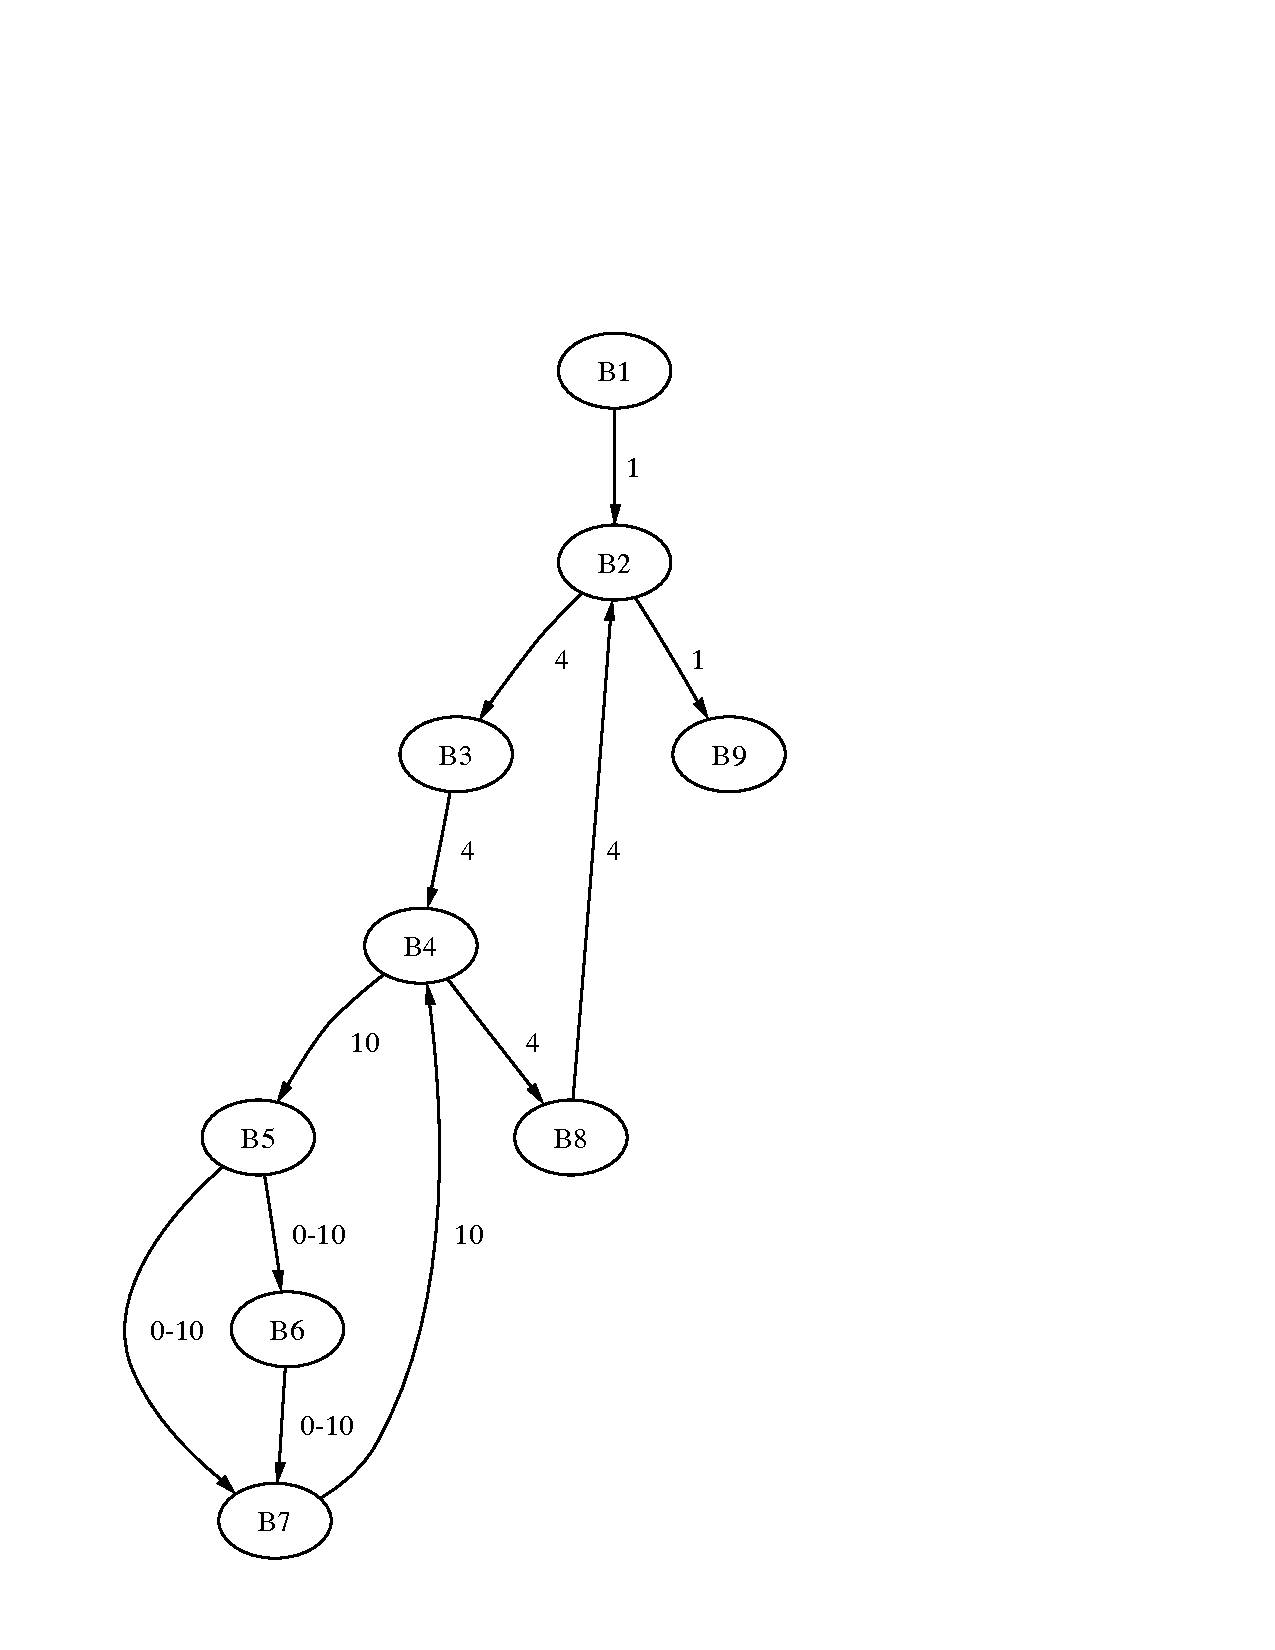
\includegraphics[height=\excelwidth]{results/results_wcet_cfg}
    \caption{The control flow graph of the Bubble Sort example}
    \label{fig:results:wcet:cfg}
\end{figure}

%The compiled version, i.e.\ the bytecodes of the test program, split
%into basic blocks, is given in
%\tablename~\ref{tab:results:bubble:wcet}. The fourth column contains
%the execution time of the bytecodes.


% the long table 'should' begin on a new page
%\pagebreak[4] %\pagebreak[3]
%{\footnotesize
%\begin{longtable}{lllr}
%    \toprule
%    Block & Addr. & Bytecode & Cycles \\
%    \midrule
%    \endhead
%    \caption{Bytecode listing of the Bubble Sort with basic blocks\label{tab:results:bubble:wcet}}
%    \endfoot
%    % table is two pages long, so don't use last caption in list
%    % of tables works
%    \caption[]{Bytecode listing of the Bubble Sort with basic blocks}
%    \endlastfoot
%    \input{bubble_instr}
%    \bottomrule
%\end{longtable}
%}


% this version fits in a two column A4 paper

%\begin{table}
%    \caption{Bytecode listing of the Bubble Sort with basic blocks}
%    \label{tab:results:bubble:wcet}
%\centering {\footnotesize
%\begin{tabular}{lllr}
%    \toprule
%    Block & Addr. & Bytecode & Cycles \\
%    \midrule
%    \input{bubble_instr}
%    \bottomrule
%\end{tabular}
%}
%\end{table}
%
\begin{table}
\centering
\begin{tabular*}{\columnwidth}{@{\extracolsep{\fill}}crrrrrr}
    \toprule
    & & &\multicolumn{2}{c}{WCET} & \multicolumn{2}{c}{BCET} \\
    Block & Addr. & Cycles & Count & Total & Count & Total \\
    \midrule
B1 & 0: &  2 &  1 &   2 &  1 &   2 \\
B2 & 2: &  5 &  5 &  25 &  5 &  25 \\
B3 & 6: &  2 &  4 &   8 &  4 &   8 \\
B4 & 8: &  6 & 14 &  84 & 14 &  84 \\
B5 &13: & 74 & 10 & 740 & 10 & 740 \\
B6 &30: & 73 & 10 & 730 &  0 &   0 \\
B7 &41: & 15 & 10 & 150 & 10 & 150 \\
B8 &47: & 15 &  4 &  60 &  4 &  60 \\
B9 &53: &    &  1 &     &  1 &     \\
\midrule
\multicolumn{4}{l}{Execution time calculated} & 1799  &    & 1069 \\
\multicolumn{4}{l}{Execution time measured}   & 1799  &    & 1069 \\
\bottomrule

\end{tabular*}
    \caption{WCET and BCET in clock cycles of the basic blocks}
    \label{tab:results:bubble:blocks}
\end{table}




In \tablename~\ref{tab:results:bubble:blocks} the basic blocks with
the start address (Addr.) and their execution time (Cycles) in clock
cycles and the worst and best case execution frequency (Count) is
given. The values in the forth and sixth columns (Count) of
\tablename~\ref{tab:results:bubble:blocks} are derived from the CFG
and show how often the basic blocks are executed in the worst and
best cases. The WCET and BCET value for each block is calculated by
multiplying the clock cycles by the execution frequency. The overall
WCET and BCET values are calculated by summing the values of the
individual blocks B1 to B8. The last block (B9) is omitted, as the
measurement does not contain the return statement.


The execution time of the program is measured using the cycle
counter in JOP. The current time is taken at both the entry of the
method and at the end, resulting in a measurement spanning from
block B1 to the beginning of block B9. The last statement, the
\code{return}, is not part of the measurement. The difference
between these two values (less the additional 8 cycles introduced by
the measurement itself) is given as the execution time in clock
cycles (the last row in \tablename~\ref{tab:results:bubble:blocks}).
The measured WCET and BCET values are exactly the same as the
calculated values.


In Figure~\ref{fig:results:wcet:sort}, the measured execution times
for all 120 permutations of the input data are shown. The vertical
axis shows the execution time in clock cycles and the horizontal
axis the number of the test run. The first input sample is an
already sorted array and results in the lowest execution time. The
last sample is the worst-case value resulting from the reversely
ordered input data. We can also see the 11 different execution times
that result from executing basic block B6 (which performs the
element exchange and takes 73 clock cycles) between 0 and 10 times.

\begin{figure}
    \centering
    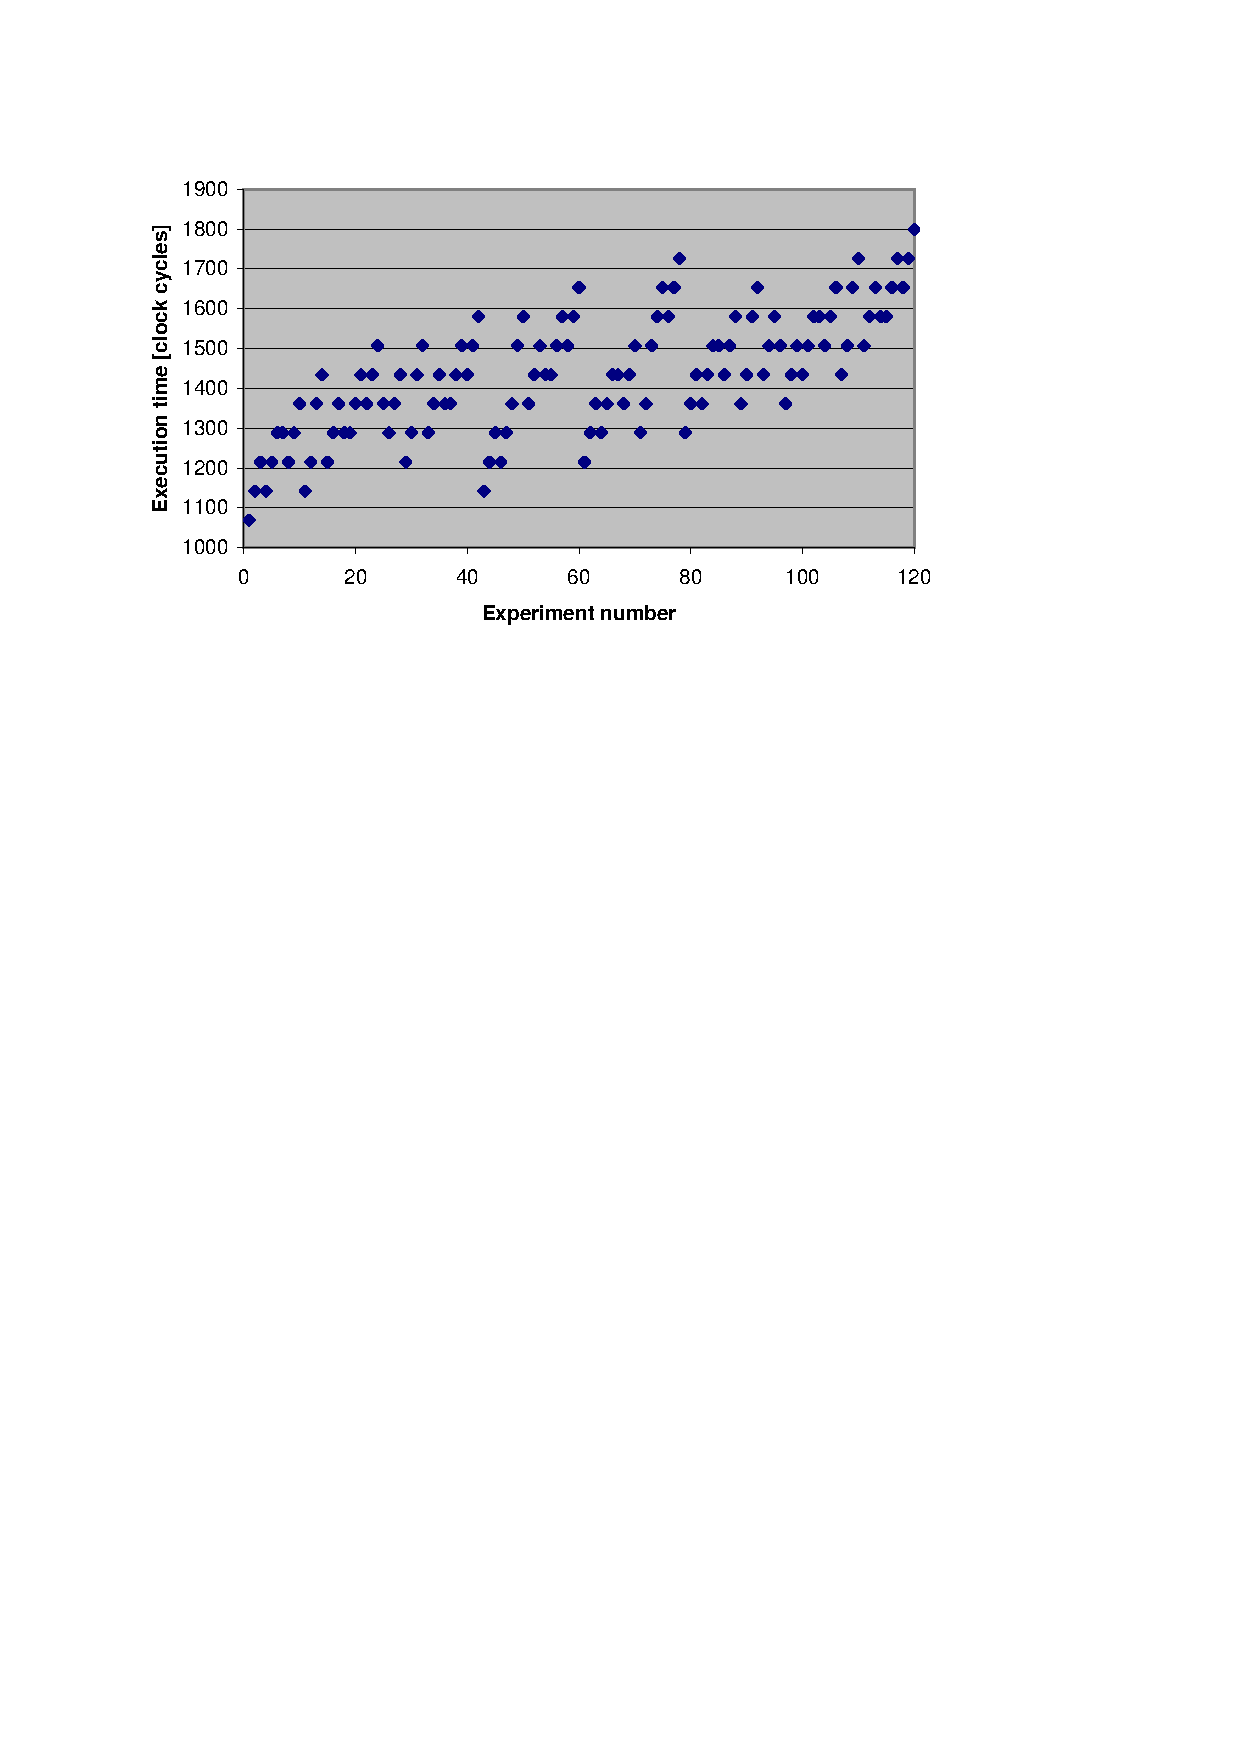
\includegraphics[width=\excelwidth]{results/results_wcet_sort}
    \caption{Execution time in clock cycles of the Bubble Sort program
    for all 120 permutations of the input data}
    \label{fig:results:wcet:sort}
\end{figure}




\subsection{WCET Analyzer} \label{sec:wcet:java}

In \cite{jop:wcet:jtres06} we have presented a static WCET analysis
tool for Java. During the high-level analysis the relevant
information is extracted from the class files. The control flow graph
(CFG) of the basic blocks\footnote{A basic block is a sequence of
instructions without any jumps or jump targets within this sequence.}
is extracted from the bytecodes. Annotations for the loop counts are
extracted from comments in the source. Furthermore, the class
hierarchy is examined to find all possible targets for a method
invoke.

The tool performs the low-level analysis at the bytecode level. The
behavior of the method cache is integrated for a simpler form (a two
block cache). The well known execution times of the different
bytecodes (see Section~\ref{sec:wcet:bc}) simplify this part of the
WCET analysis, which is usually the most complex one, to a great
extent. As there are no pipeline dependencies, the calculation of the
execution time for a basic block is merely just adding the individual
cycles for each instruction.

The actual calculation of the WCET is transformed to an integer
linear programming problem, a well known technique for WCET analysis
\cite{Puschner:JRTS1997,216666}. We performed the WCET analysis on
several benchmarks (see Table~\ref{tab:examples}). We also
\emph{measured} the WCET values for the benchmarks. It has to be
noted that we actually cannot measure the real WCET. If we could
measure it, we would not need to perform the WCET analysis at all.
The measurement gives us an idea of the pessimism of the analyzed
WCET.
%
\begin{table}
\centering {
\begin{tabular*}{\columnwidth}{@{\extracolsep{\fill}}llr}
    \toprule
    Program & Description & LOC \\
    \midrule
    \code{crc} & CRC calculation for short messages & 8 \\
    \code{robot} & A simple line follower robot & 111 \\
    \code{Lift} & A lift controler & 635 \\
    \code{Kfl} & \emph{Kippfahrleitung} application & 1366 \\
    \code{UdpIp} & UDP/IP benchmark & 1297 \\
    \bottomrule
\end{tabular*}
}
    \caption{WCET benchmark examples}
    \label{tab:examples}
\end{table}
%
The benchmarks \code{Lift} and \code{Kfl} are real-world examples
that are in industrial use. \code{Kfl} and \code{UdpIp} are also part
of an embedded Java benchmark suite that is used in
Section~\ref{sec:performance}.

Table~\ref{tab:wcet:compared} shows the measured execution time and
the analyzed WCET. The last column gives an idea of the pessimism of
the WCET analysis. For very simple programs, such as \code{crc} and
\code{robot}, the pessimism is quite low. For the \code{Lift}
example it is in an acceptable range.
%
\begin{table}
\centering {
\begin{tabular*}{\columnwidth}{@{\extracolsep{\fill}}lrrr}
    \toprule
%    & \multicolumn{2}{c}{WCET} & \\
            & Measured & Estimated & Pessimism\\
    Program & (cycle) & (cycle) & (ratio)\\
    \midrule
    \code{crc} & 1552 & 1620 & 1.04 \\
    \code{robot} & 736 & 775 & 1.05 \\
    \code{Lift} & 7214 & 11249 & 1.56 \\
    \code{Kfl} & 13334 & 28763 & 2.16 \\
    \code{UdpIp} & 11823 & 219569 & 18.57 \\
    \bottomrule
\end{tabular*}
}
    \caption{Measured and estimated WCETs with results in clock cycles}
    \label{tab:wcet:compared}
\end{table}
%
The difference between the measurement and the analysis in the
\code{Kfl} example results from the fact that our measurement does
not cover the WCET path. The large conservatism in \code{UdpIp}
results from the loop bound in the IP and UDP checksum calculation.
It is set for a 1500 byte packet buffer, but the payload in the
benchmark is only 8 bytes. The last two examples also show the issue
when a real-time application is developed without a WCET analysis
tool available.

The WCET analysis tool, with the help of loop annotations, provides
WCET values for the schedulability analysis. Besides the calculation
of the WCET, the tool provides user feedback by generating bytecode
listings with timing information and a graphical representation of
the CFG with timing and frequency information. This representation of
the WCET path through the code can guide the developer to write WCET
aware real-time code.

\section{Discussion}

The Bubble Sort example and experiments with the WCET analyzer tool
have demonstrated that we have achieved our goal: JOP is a simple
target for the WCET analysis. Most bytecodes have a single execution
time (WCET = BCET), and the WCET of a task (the analysis at the
bytecode level) depends only on the control flow. No pipeline or
data dependencies complicate the low-level part of the WCET
analysis.


The same analysis is not possible for other Java processors. Either
the information on the bytecode execution time is missing\footnote{We
tried hard to get this information for the aJile processor.} or some
processor features (e.g., the high variability of the latency for a
trap in picoJava) would result in very conservative WCET estimates.
Another example that prohibits exact analysis is the mechanism to
automatically fill and spill the stack cache in picoJava. The time
when the memory (cache) is occupied by this spill/fill action depends
on a long instruction history. Also the fill level of the
16-byte-deep prefetch buffer, which is needed for instruction
folding, depends on the execution history. All these automatic
buffering features have to be modeled quite conservatively. A
pragmatic solution is to assume empty buffers at the start of a basic
block. As basic blocks are quite short, most of the
buffering/prefetching does not help to lower the WCET.

Only for the Cjip processor is the execution time well documented
\cite{CjipRef}. However, as seen in Section~\ref{sec:perf:disc}, the
\emph{measured} execution time of some bytecodes is \emph{higher}
than the documented values. Therefore the documentation is not
complete to provide a safe processor model of the Cjip for the WCET
analysis.
